% !TEX TS-program = pdflatex
% !TEX encoding = UTF-8 Unicode

% This is a simple template for a LaTeX document using the "article" class.
% See "book", "report", "letter" for other types of document.

\documentclass[11pt]{article} % use larger type; default would be 10pt

\usepackage[utf8]{inputenc} % set input encoding (not needed with XeLaTeX)
\usepackage{graphicx}
\usepackage{algorithm}
\usepackage{algorithmicx}
\usepackage{algpseudocode}
\usepackage{multirow}\usepackage{listings}
\usepackage{color}
\usepackage{textcomp}
\definecolor{listinggray}{gray}{0.9}
\definecolor{lbcolor}{rgb}{0.9,0.9,0.9}
\lstset{
    language=java,
    basicstyle=\scriptsize,
    upquote=true,
    aboveskip={1.5\baselineskip},
    columns=fullflexible,
    showstringspaces=false,
    extendedchars=true,
    breaklines=true,
    showtabs=false,
    showspaces=false,
    showstringspaces=false,
    identifierstyle=\ttfamily,
    keywordstyle=\color[rgb]{0,0,1},
    commentstyle=\color[rgb]{0.133,0.545,0.133},
    stringstyle=\color[rgb]{0.627,0.126,0.941},
}

%%% Examples of Article customizations
% These packages are optional, depending whether you want the features they provide.
% See the LaTeX Companion or other references for full information.

%%% PAGE DIMENSIONS
\usepackage{geometry} % to change the page dimensions
\geometry{a4paper} % or letterpaper (US) or a5paper or....
% \geometry{margin=2in} % for example, change the margins to 2 inches all round
% \geometry{landscape} % set up the page for landscape
%   read geometry.pdf for detailed page layout information

\usepackage{graphicx} % support the \includegraphics command and options

% \usepackage[parfill]{parskip} % Activate to begin paragraphs with an empty line rather than an indent

%%% PACKAGES
\usepackage{booktabs} % for much better looking tables
\usepackage{array} % for better arrays (eg matrices) in maths
\usepackage{paralist} % very flexible & customisable lists (eg. enumerate/itemize, etc.)
\usepackage{verbatim} % adds environment for commenting out blocks of text & for better verbatim
\usepackage{subfig} % make it possible to include more than one captioned figure/table in a single float
% These packages are all incorporated in the memoir class to one degree or another...

%%% HEADERS & FOOTERS
\usepackage{fancyhdr} % This should be set AFTER setting up the page geometry
\pagestyle{fancy} % options: empty , plain , fancy
\renewcommand{\headrulewidth}{0pt} % customise the layout...
\lhead{}\chead{}\rhead{}
\lfoot{}\cfoot{\thepage}\rfoot{}

%%% SECTION TITLE APPEARANCE
\usepackage{sectsty}
\allsectionsfont{\sffamily\mdseries\upshape} % (See the fntguide.pdf for font help)
% (This matches ConTeXt defaults)

%%% ToC (table of contents) APPEARANCE
\usepackage[nottoc,notlof,notlot]{tocbibind} % Put the bibliography in the ToC
\usepackage[titles,subfigure]{tocloft} % Alter the style of the Table of Contents
\renewcommand{\cftsecfont}{\rmfamily\mdseries\upshape}
\renewcommand{\cftsecpagefont}{\rmfamily\mdseries\upshape} % No bold!

%%% END Article customizations

%%% The "real" document content comes below...

\title{Lab 6: Clustering and Community Detection}
\author{Ruofan Zhou}
%\date{} % Activate to display a given date or no date (if empty),
         % otherwise the current date is printed 

\begin{document}
\maketitle

\section{Clustering}

\subsection{codes}

1. mStep of Kmeans:
\begin{lstlisting}
public void mStep() {
        // According to the assignment, we update the center of each cluster
    	for (int c = 0; c < this.k; ++c) {
    		Point2d rnk = new Point2d(0, 0);
    		double sum = 0.0;
    		for (int p = 0; p < this.data.length; ++p) {
    			if (this.assignments[p] == c) {
    				sum = sum + 1;
    				rnk.set(rnk.getX() + this.data[p].getX(), rnk.getY() + this.data[p].getY());
    			}
    		}
    		this.centers[c].set(rnk.getX() / sum, rnk.getY() / sum);
    	}
    }
\end{lstlisting}
2. mStep \& eStep of Kmeans:
\begin{lstlisting}
public void eStep() {
        // Hint: look at the MultivariateNormalDistribution class used in logLikelihood
    	MultivariateNormalDistribution[] pdfs = new MultivariateNormalDistribution[this.k];
        for (int c = 0; c < this.k; c++) {
            pdfs[c] = new MultivariateNormalDistribution(this.mus[c].toArray(),
                    this.sigmas[c].toArray());
        }
        for (int p = 0; p < this.data.length; ++p) {
        	double sum = 0.0;
        	for (int c = 0; c < this.k; ++c) {
        		sum += pdfs[c].density(this.data[p].toArray()) * this.pi[c];
        	}
        	for (int c = 0; c < this.k; ++c) {
        		this.gamma[p][c] = this.pi[c] * pdfs[c].density(this.data[p].toArray()) / sum;
        	}
        }
    }

public void mStep() {
    	for (int c = 0; c < this.k; ++c) {
    		double Nsum = 0.0;
    		//compute mus
    		this.mus[c].set(0.0, 0.0);
    		for (int i = 0; i < this.data.length; ++i) {
    			Nsum = Nsum + gamma[i][c];
    			this.mus[c].set(this.mus[c].getX() + gamma[i][c] * this.data[i].getX(),
    					this.mus[c].getY() + gamma[i][c] * this.data[i].getY());
    		}
    		this.mus[c].set(this.mus[c].getX() / Nsum, this.mus[c].getY() / Nsum);
    		
    		double x = 0.0, y = 0.0, xy = 0.0;
    		for (int i = 0; i < this.data.length; ++i) {
    			double a = this.data[i].getX() - this.mus[c].getX();
    			double b = this.data[i].getY() - this.mus[c].getY();
    			x += a * a * this.gamma[i][c];
    			y += b * b * this.gamma[i][c];
    			xy += a * b * this.gamma[i][c];
    		}
    		this.sigmas[c].set(x / Nsum, y / Nsum, xy / Nsum);    		
    		this.pi[c] = Nsum / this.data.length;
    	}    	
    }
\end{lstlisting}

\subsection{answers to the questions}

1.  The plot of tweet by K-means is below. The geographical distribution of the clusters shows nothing with Manhattan.
\\
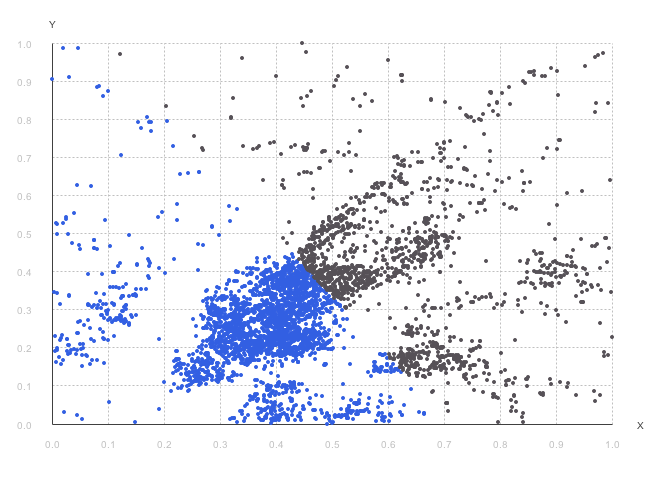
\includegraphics[width=10cm]{kmean-tweet}\\
2. The measure used in GMM that is the equivalent of the distortion measure in k-means is \emph{LogLikelihood}.\\
3. GMM plots for tweet are as below:\\
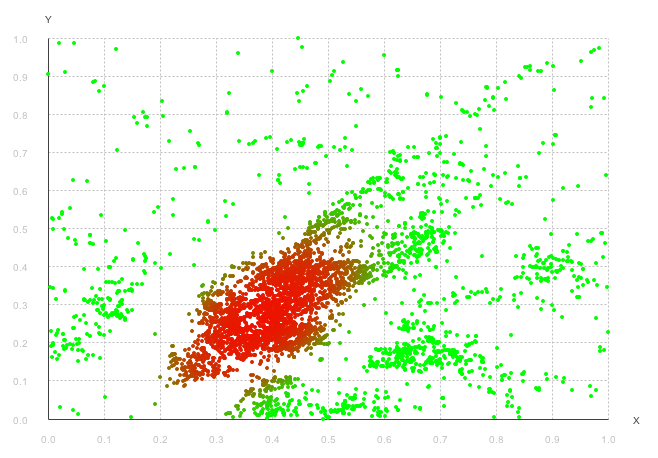
\includegraphics[width=8cm]{gauss-tweet2}\\
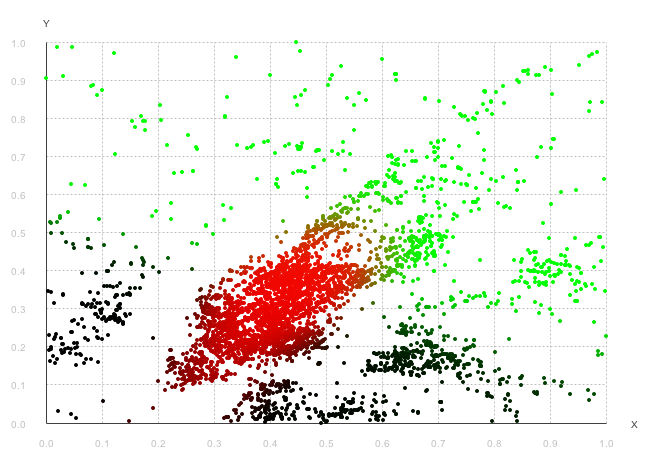
\includegraphics[width=8cm]{gauss-tweet3}\\
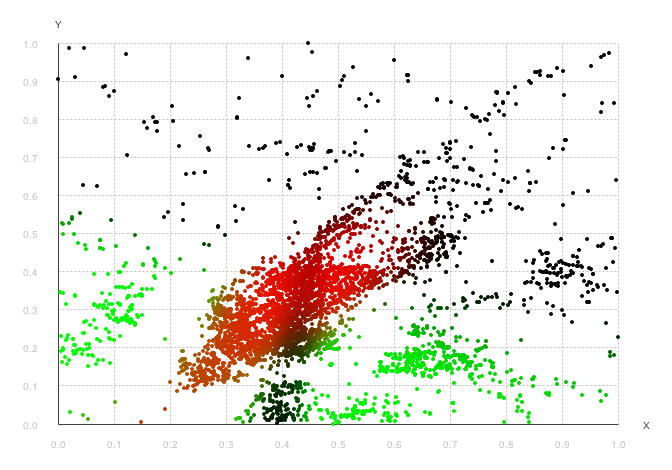
\includegraphics[width=8cm]{gauss-tweet4}\\

\section{Community Detection}
\subsection{codes}
communityDetection() of Louvain:
\begin{lstlisting}
public void communityDetection() {
    	double delta = 0.0;
    	int level = 0;
    	do {
    		Status s = statusList.get(level ++);
    		s.assignCommunities();
    		Status s1 = s.getNextLevel();
    		statusList.add(s1);
    		delta = s1.modularity() - s.modularity();
    	} while (delta > CHANGE_MIN);
    	System.out.println(statusList.get(level).modularity());
    }
\end{lstlisting}

\subsection{plots}
1. Plot of the simple graph and the communities found at the first level of the Louvain method:\\
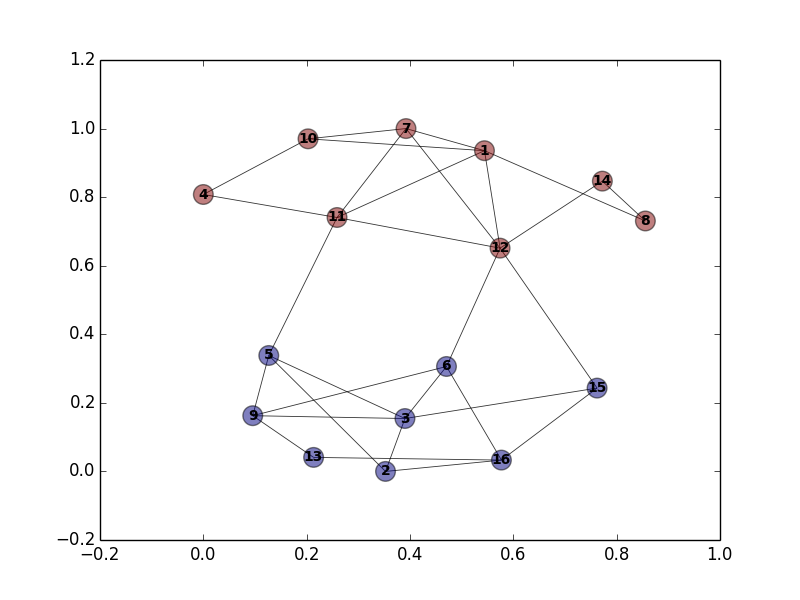
\includegraphics[width=10cm]{simple-gra}\\

2. Plot of the karate graph and the best communities found by the Louvain method:\\
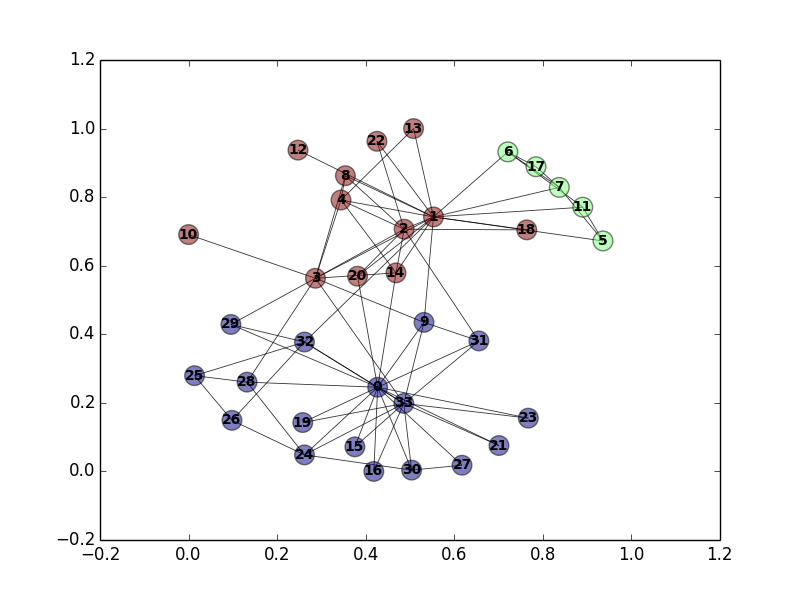
\includegraphics[width=10cm]{karate-gra}\\

3. Highest modularity of the wikipedia graph found by the Louvain method is \emph{0.5236077874099563}.\\

4. Plot of communities of the node Google and its neighbors from the wikipedia graph:\\
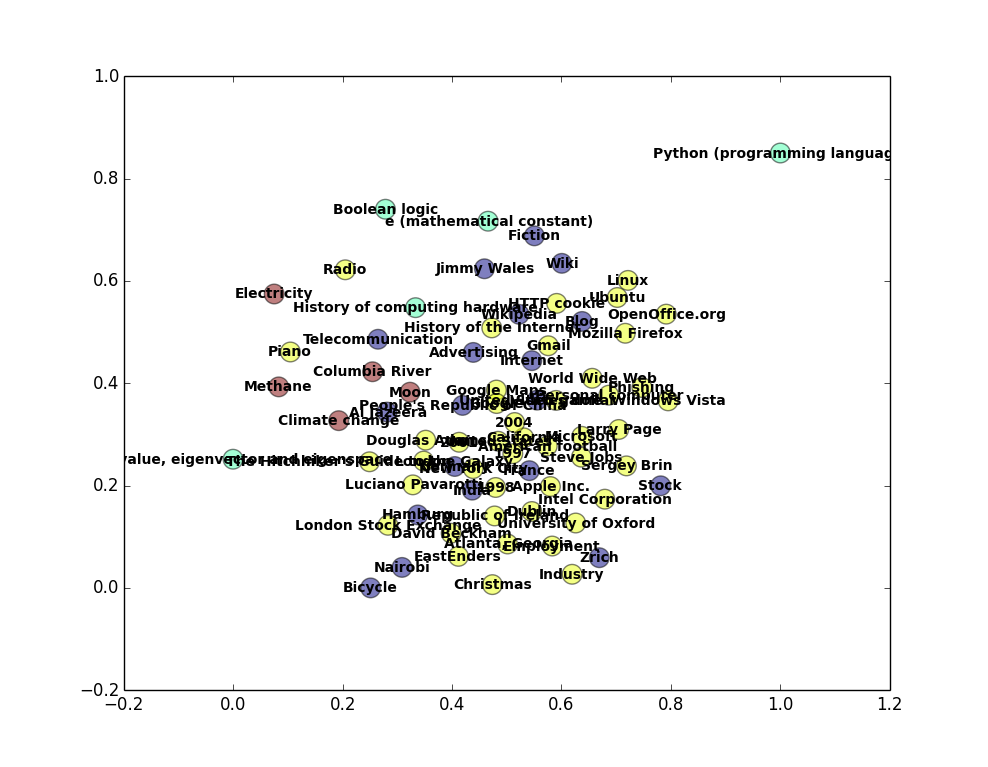
\includegraphics[width=10cm]{google_nei}\\

%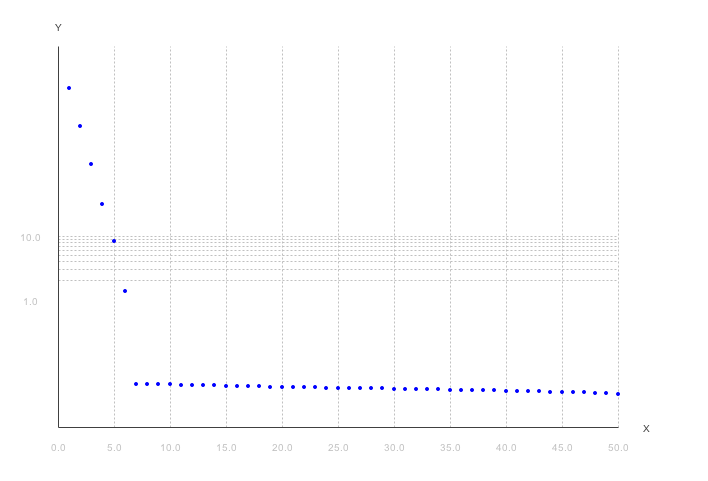
\includegraphics[width=10cm]{pic/p3}}
\end{document}
